\documentclass[fleqn, a4paper, 12pt, twoside]{article}
\usepackage{exsheets} %question and solution environments
\usepackage{amsmath, amssymb, amsthm} %standard AMS packages
\usepackage{esint} %integral signs
\usepackage{marginnote} %marginnotes
\usepackage{gensymb} %miscellaneous symbols
\usepackage{commath} %differential symbols
\usepackage{xcolor} %colours
\usepackage{cancel} %cancelling terms
\usepackage{siunitx} %formatting units
\usepackage{tikz, pgfplots} %diagrams
	\usetikzlibrary{calc, hobby, patterns, intersections, angles, quotes, spy}
\usepackage{graphicx} %inserting graphics
\usepackage{epstopdf} %converting and inserting eps graphics
\usepackage{hyperref} %hyperlinks
\usepackage{datetime} %date and time
\usepackage{ulem} %underline for \emph{}
\usepackage{xfrac, lmodern} %inline fractions
\usepackage{enumerate, enumitem} %numbered lists
\usepackage{float} %inserting floats
\usepackage[american voltages]{circuitikz} %circuit diagrams
\usepackage{pdflscape} %pages in landscape orientation
\usepackage{setspace} %double spacing
\usepackage{microtype} %micro-typography
\usepackage{listings} %formatting code
	\lstset{language=Matlab}
	\lstdefinestyle{standardMatlab}
	{
		belowcaptionskip=1\baselineskip,
		breaklines=true,
		frame=L,
		xleftmargin=\parindent,
		language=C,
		showstringspaces=false,
		basicstyle=\footnotesize\ttfamily,
		keywordstyle=\bfseries\color{green!40!black},
		commentstyle=\itshape\color{purple!40!black},
		identifierstyle=\color{blue},
		stringstyle=\color{orange},
	}
\usepackage{algpseudocode} %algorithms
\usepackage{algorithm} %algorithms
\usepackage{environ}
\usepackage{todonotes}

\renewcommand{\marginfont}{\scriptsize \color{red}}

\newcommand\numberthis{\addtocounter{equation}{1}\tag{\theequation}} %adds numbers to specific equations in non-numbered list of equations

\theoremstyle{definition}
\newtheorem{example}{Example}
\newtheorem{definition}{Definition}

\theoremstyle{theorem}
\newtheorem{theorem}{Theorem}
\newtheorem{law}{Law}

\newcommand{\curl}{\mathrm{curl\,}}

\newcommand{\divergence}{\mathrm{div\,}}

\newcommand{\dist}{\mathrm{d}}

\newcommand{\normeq}{\stackrel{\|\cdot\|}{=}}

\makeatletter
\@addtoreset{section}{part} %resets section numbers in new part
\makeatother

\newcommand\blfootnote[1]{%
	\begingroup
	\renewcommand\thefootnote{}\footnote{#1}%
	\addtocounter{footnote}{-1}%
	\endgroup
}

\renewcommand{\tilde}{\widetilde}

\SetupExSheets{solution/print = true} %prints all solutions by default

% Uncomment to hide proofs
%\NewEnviron{killcontents}{}
%\let\proof\killcontents
%\let\endproof\endkillcontents

%opening
\title{Harmonic Analysis : Review Session}
\author{Aakash Jog}
\date{2015-16}

\begin{document}

\maketitle
%\setlength{\mathindent}{0pt}

\blfootnote
{	
	\begin{figure}[H]
		
\includegraphics[height = 12pt]{cc.eps}
		
\includegraphics[height = 12pt]{by.eps}
		\includegraphics[height = 12pt]{nc.eps}
		
\includegraphics[height = 12pt]{sa.eps}
	\end{figure}
	This work is licensed under the Creative Commons Attribution-NonCommercial-ShareAlike 4.0 International License. To view a copy of this license, visit \url{http://creativecommons.org/licenses/by-nc-sa/4.0/}.
} %CC-BY-NC-SA license

\tableofcontents

\newpage

\begin{question}
	Is $\left\{ 1,\cos(n x) \right\}$ orthogonal and complete in $L^2[0,\pi]$?
\end{question}

\begin{solution}
	$L^2[0,\pi]$ is the inner product space of all functions defined on the interval $[0,\pi]$ with inner product.\\
	For all $f(x)$, let
	\begin{align*}
		F(x) &=
			\begin{cases}
				f(x)  & ;\quad 0 \le x \le \pi  \\
				f(-x) & ;\quad -\pi \le x \le 0 \\
			\end{cases}
	\end{align*}
	Therefore, $F(x)$ is even.
	Therefore, the Fourier series of $F(x)$ will be of the form
	\begin{align*}
		F(x) & \approx \frac{a_0}{2} + \sum\limits_{n = 1}^{\infty} a_n \cos(n x)
	\end{align*}
	Therefore, as $\left\{ \frac{1}{\sqrt{2}},\sin(n x),\cos(n x) \right\}$ is complete and orthogonal in $L^2[-\pi,\pi]$.\\
	Therefore, for any $f \in L^2[0,\pi]$, and its equivalent $F(x)$, the function can be described with $\left\{ \frac{1}{\sqrt{2}},\cos(n x) \right\}$.
	Therefore, the set $\left\{ \frac{1}{\sqrt{2}},\cos(n x) \right\}$ is orthonormal and complete.\\
	Hence, the set $\left\{ 1,\cos(n x) \right\}$ is orthogonal and complete in $L^2[0,\pi]$.
\end{solution}

\end{document}
